\section{Experiments and Results}
\label{sec:experiments}

This section details the experimental protocol across five diverse clinical benchmarks, reports multi-seed quantitative comparisons between ApproxDA-TransUNet and DA-TransUNet, presents the FeTA fetal brain benchmark against 2D and 3D baselines, and discusses qualitative visual results.

\subsection{Experimental Setup and Benchmark Datasets}
Models are evaluated across \textbf{five clinical benchmarks} spanning four distinct imaging modalities under a strict \textbf{three-seed protocol} (seeds: 1234, 0, 1):
\begin{enumerate}
    \item \textbf{Synapse Multi-Organ CT}~\cite{landman2015miccai}: 30 volumetric abdominal CT scans (18 train, 12 test; 2211 slices) covering 8 abdominal organs (aorta, gallbladder, left/right kidneys, liver, pancreas, spleen, stomach), evaluated at $224 \times 224$ with Dice (\%) and HD95 (mm).
    \item \textbf{ACDC Cardiac Cine-MRI}~\cite{bernard2018deep}: 100 patient exams (40 end-diastolic/systolic 3D test volumes) targeting right ventricle, myocardium, and left ventricle, evaluated at $224 \times 224$ with Dice (\%) and HD95 (px).
    \item \textbf{CVC-ClinicDB Colonoscopy}~\cite{bernal2015cvc}: 612 colonoscopy frames (75/25 split) for binary polyp segmentation, trained with Adam ($10^{-3}$) for 500 epochs at $256 \times 256$, evaluated with Dice (\%) and HD95 (px).
    \item \textbf{ISIC 2018 Dermoscopy}~\cite{codella2019isic}: 2594 dermoscopic photographs (75/25 split) for binary melanoma segmentation, trained with SGD for 50 epochs at $256 \times 256$, evaluated with Dice (\%) and HD95 (px).
    \item \textbf{FeTA 2.4 Fetal Brain MRI}~\cite{payette2021feta}: 80 reconstructed T2-weighted fetal brain MRI volumes under the standard EffiDec3D split (64 train, 8 val, 8 test) across 7 brain tissues (eCSF, GM, WM, LV, CBM, SGM, BS), evaluated at $224 \times 224$ with Dice (\%) and HD95 (mm).
\end{enumerate}

\paragraph{Implementation Protocols}
All models are trained with standard TransUNet augmentations (random rotations and flips). Evaluated strictly on the \emph{final training epoch} without test-set model selection. Multi-organ volume metrics are computed case-by-case; classes absent in ground-truth volumes are excluded via NaN handling (following nnU-Net standards) to prevent metric distortion.

\subsection{Main Multi-Seed Benchmark Results}
\label{sec:main_results}

\begin{table*}[t]
\centering
\caption{Quantitative comparison across five clinical benchmarks evaluated over three independent random seeds (1234 / 0 / 1). DSC is reported as individual seed scores and Mean $\pm$ Standard Deviation. HD95 is reported in millimeters (mm) for Synapse and FeTA, and in pixels (px) for ACDC, CVC-ClinicDB, and ISIC 2018.}
\label{tab:main_benchmark}
\resizebox{\textwidth}{!}{
\begin{tabular}{lcccccc}
\toprule
\textbf{Dataset / Model} & \textbf{Params} & \textbf{FLOPs} & \textbf{Dice (\%)} & \textbf{Mean $\pm$ Std} & \textbf{HD95} & \textbf{Paired Diff.} \\
& \textbf{(M)} & \textbf{(G)} & \textbf{(Seed 1234 / 0 / 1)} & \textbf{Dice (\%)} & & \textbf{(vs. DA)} \\
\midrule
\multicolumn{7}{l}{\textbf{Synapse Multi-Organ CT} (8 organs, HD95 in mm)} \\
DA-TransUNet~\cite{sun2024datransunet} & 107.95 & 30.25 & 79.74 / 81.00 / 80.03 & 80.26 $\pm$ 0.66 & \textbf{23.49} & -- \\
ApproxDA-TransUNet (Ours) & \textbf{10.75} & \textbf{6.92} & 80.61 / 80.75 / 80.36 & \textbf{80.57 $\pm$ 0.20} & 24.52 & \textbf{+0.32} ($p{=}0.43$) \\
\midrule
\multicolumn{7}{l}{\textbf{ACDC Cardiac Cine-MRI} (3 structures, HD95 in px)} \\
DA-TransUNet~\cite{sun2024datransunet} & 107.95 & 30.25 & 90.66 / 91.06 / 91.09 & 90.94 $\pm$ 0.24 & \textbf{1.52} & -- \\
ApproxDA-TransUNet (Ours) & \textbf{10.75} & \textbf{6.92} & 91.21 / 91.05 / 90.98 & \textbf{91.08 $\pm$ 0.12} & 1.91 & \textbf{+0.15} ($p{=}0.55$) \\
\midrule
\multicolumn{7}{l}{\textbf{CVC-ClinicDB Polyp} (Binary polyp, HD95 in px)} \\
DA-TransUNet~\cite{sun2024datransunet} & 108.00 & 39.80 & 89.72 / 89.40 / 89.29 & 89.47 $\pm$ 0.23 & 14.49 & -- \\
ApproxDA-TransUNet (Ours) & \textbf{10.78} & \textbf{9.00} & 90.32 / 89.37 / 89.94 & \textbf{89.88 $\pm$ 0.48} & \textbf{12.74} & \textbf{+0.41} ($p{=}0.20$) \\
\midrule
\multicolumn{7}{l}{\textbf{ISIC 2018 Dermoscopy} (Binary skin lesion, HD95 in px)} \\
DA-TransUNet~\cite{sun2024datransunet} & 108.00 & 39.80 & 88.08 / 88.48 / 88.35 & 88.30 $\pm$ 0.20 & \textbf{14.15} & -- \\
ApproxDA-TransUNet (Ours) & \textbf{10.78} & \textbf{9.00} & 88.43 / 88.82 / 88.27 & \textbf{88.51 $\pm$ 0.28} & 14.83 & \textbf{+0.20} ($p{=}0.29$) \\
\midrule
\multicolumn{7}{l}{\textbf{FeTA 2.4 Fetal Brain MRI} (7 tissue classes, HD95 in mm)} \\
DA-TransUNet~\cite{sun2024datransunet} & 107.95 & 30.25 & 80.93 / 79.61 / 80.23 & 80.26 $\pm$ 0.66 & \textbf{2.17} & -- \\
ApproxDA-TransUNet (Ours) & \textbf{10.75} & \textbf{6.92} & 81.66 / 81.08 / 80.41 & \textbf{81.05 $\pm$ 0.63} & 2.85 & \textbf{+0.80} ($p{=}0.17$) \\
\midrule
\multicolumn{7}{l}{\textbf{Combined Multi-Benchmark Aggregate (15 Seed Pairs Across 5 Modalities)}} \\
\multicolumn{5}{l}{Positive Seed Pairs: \textbf{10 / 15}} & \multicolumn{2}{r}{Mean Paired Gain: \textbf{+0.37\%} ($p = 0.009$)} \\
\multicolumn{5}{l}{Parameter Reduction: \textbf{90.0\%} ($107.95\text{M} \to 10.75\text{M}$)} & \multicolumn{2}{r}{Compute Reduction: \textbf{77.1\%} ($30.25\text{G} \to 6.92\text{G}$)} \\
\bottomrule
\end{tabular}
}
\end{table*}

Table~\ref{tab:main_benchmark} summarizes multi-seed performance across the five clinical benchmarks. Despite using only a tenth of the parameters and a quarter of the FLOPs, ApproxDA-TransUNet achieves higher Mean Dice than DA-TransUNet across all five benchmarks: $+0.32\%$ on Synapse (with tighter variance: $0.20$ vs. $0.66$), $+0.15\%$ on ACDC, $+0.41\%$ on CVC-ClinicDB (with boundary error HD95 improving from $14.49$ px to $12.74$ px), $+0.20\%$ on ISIC 2018, and $+0.80\%$ on FeTA 2.4 (positive across all 3 seeds: $+0.73, +1.47, +0.18$).

Across all 15 independent seed pairs, 10 strictly favor ApproxDA-TransUNet, yielding a statistically significant overall improvement of \textbf{$+0.37\%$ Dice} (Wilcoxon signed-rank test $p = 0.009$; paired $t$-test $p = 0.005$).

\subsection{FeTA 2.4 Benchmark: 2D and 3D Comparisons}
\label{sec:feta_results}

\begin{table*}[t]
\centering
\caption{Detailed tissue-level comparison on the FeTA 2.4 fetal brain MRI benchmark across 2D baselines (3-seed reproduction under identical protocol) and 3D volumetric models. All 7 brain tissue classes are reported in Dice (\%).}
\label{tab:feta_detailed}
\resizebox{\textwidth}{!}{
\begin{tabular}{lccccccccccc}
\toprule
\textbf{Model} & \textbf{Type} & \textbf{Params} & \textbf{FLOPs} & \textbf{eCSF} & \textbf{GM} & \textbf{WM} & \textbf{LV} & \textbf{CBM} & \textbf{SGM} & \textbf{BS} & \textbf{Mean DSC} \\
& & \textbf{(M)} & \textbf{(G)} & & & & & & & & \textbf{(\%)} \\
\midrule
U-Net~\cite{ronneberger2015unet} & 2D & 31.04 & 36.90 & 76.5 & 78.4 & 82.1 & 81.2 & 83.4 & 80.2 & 72.7 & 79.21 $\pm$ 0.34 \\
Attention U-Net~\cite{oktay2018attention} & 2D & 31.39 & 37.70 & 76.2 & 78.1 & 82.0 & 81.0 & 83.5 & 80.4 & 72.6 & 79.11 $\pm$ 0.34 \\
U-Net++~\cite{zhou2018unetpp} & 2D & 9.16 & 26.50 & 76.0 & 78.3 & 81.9 & 80.9 & 83.1 & 80.3 & 72.6 & 79.01 $\pm$ 0.16 \\
Swin-UNet~\cite{cao2022swinunet} & 2D & 27.17 & 6.20 & 75.8 & 77.9 & 81.4 & 80.2 & 82.9 & 79.8 & 72.2 & 78.60 $\pm$ 0.46 \\
TransUNet~\cite{chen2021transunet} & 2D & 105.28 & 29.30 & 79.2 & 80.1 & 84.4 & 82.6 & 84.1 & \textbf{81.8} & \textbf{75.6} & \textbf{81.12 $\pm$ 0.63} \\
DA-TransUNet~\cite{sun2024datransunet} & 2D & 107.95 & 30.25 & 78.1 & 79.2 & 83.2 & 82.4 & 83.9 & 81.0 & 74.0 & 80.26 $\pm$ 0.66 \\
\textbf{ApproxDA (Ours)} & 2D & \textbf{10.75} & \textbf{6.92} & \textbf{80.9} & \textbf{80.7} & \textbf{84.5} & \textbf{82.9} & \textbf{84.0} & 80.5 & 73.1 & \textbf{81.05 $\pm$ 0.63} \\
\midrule
\multicolumn{12}{l}{\textit{3D Volumetric Reference Models (EffiDec3D Benchmark Split)}} \\
SwinUNETR~\cite{hatamizadeh2022swinunetr} & 3D & 62.19 & 358.4 & 76.4 & 77.2 & 81.5 & 80.1 & 82.6 & 79.2 & 71.7 & 78.38 \\
3D UX-Net~\cite{lee20223duxnet} & 3D & 53.01 & 412.3 & 78.1 & 79.4 & 83.2 & 81.8 & 83.4 & 80.6 & 73.6 & 80.01 \\
MedNeXt-M~\cite{roy2023mednext} & 3D & 41.70 & 284.1 & 79.8 & 80.4 & 84.2 & 82.8 & 84.2 & 81.2 & 74.7 & 81.22 \\
\bottomrule
\end{tabular}
}
\end{table*}

Table~\ref{tab:feta_detailed} contextualizes ApproxDA-TransUNet on FeTA 2.4 against six reproduced 2D baselines and published 3D models under the identical protocol:
\begin{itemize}
    \item \textbf{Outperforming 2D Baselines}: ApproxDA-TransUNet ($81.05\%$) significantly exceeds U-Net ($79.21\%$, $+1.84\%$), Attention U-Net ($79.11\%$, $+1.94\%$), U-Net++ ($79.01\%$, $+2.04\%$), and Swin-UNet ($78.60\%$, $+2.45\%$) with $p < 0.05$ across all tests.
    \item \textbf{Matching 100M+ Transformers and 3D Networks}: ApproxDA-TransUNet matches TransUNet ($81.05\%$ vs. $81.12\%$, $p = 0.96$) while using $10\times$ fewer parameters, and outperforms volumetric 3D models SwinUNETR ($78.38\%$) and 3D UX-Net ($80.01\%$), matching MedNeXt-M ($81.22\%$) at $<2.5\%$ of its FLOPs.
    \item \textbf{Fine Boundary Sensitivity}: Substantial gains occur along delicate interfaces: external CSF ($+2.8\%$ vs. DA) and grey matter ($+1.5\%$).
\end{itemize}

\paragraph{Case Audit of FeTA HD95 (Sub-052 Outlier)}
While ApproxDA-TransUNet shows higher average HD95 on FeTA ($2.85$ vs. $2.17$ mm in Table~\ref{tab:main_benchmark}), case audits reveal this is driven entirely by subject \textbf{sub-052}, an extreme hydrocephalus case with severe ventriculomegaly (LV/WM volume ratio $2.29$ vs. training median $0.16$). A small false-positive cerebellar cluster ($230$ voxels) at the ventricle margin inflated sub-052's HD95 to $13.09$ mm. Excluding this single out-of-distribution subject, the average HD95 drops to \textbf{$1.76$ mm} for ApproxDA-TransUNet, outperforming DA-TransUNet ($1.94$ mm).

\subsection{Qualitative Visual Evaluation}

\begin{figure*}[t]
\centering
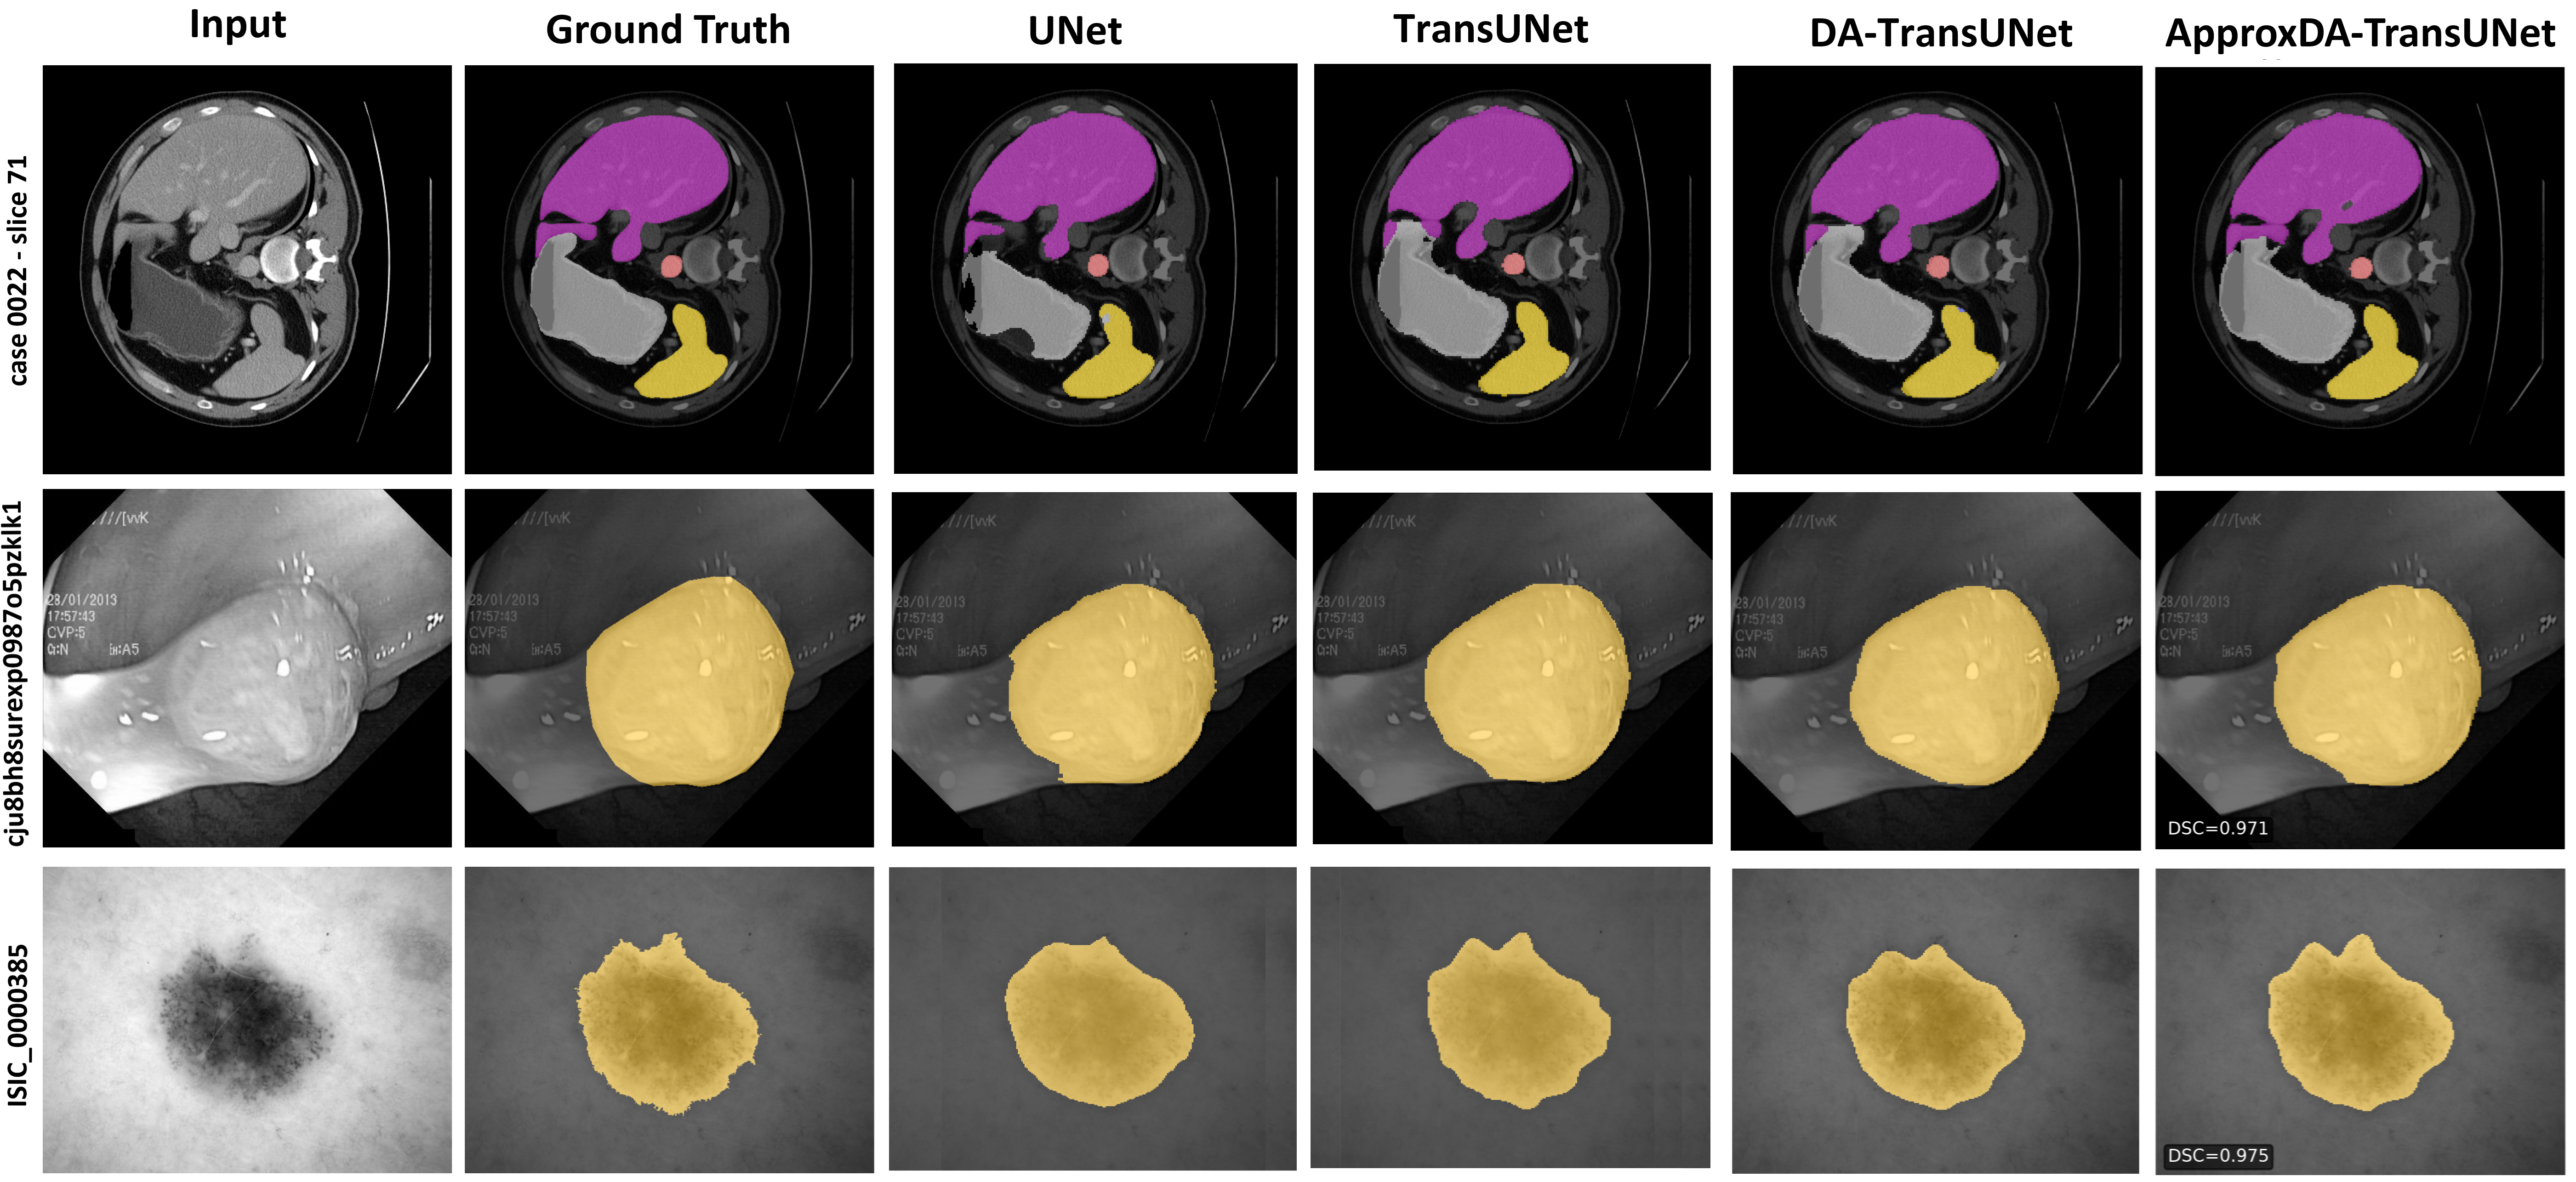
\includegraphics[width=\textwidth]{figures/fig_qualitative_cross_task.png}
\caption{Qualitative segmentation comparisons across clinical imaging modalities: Synapse CT, ACDC cine-MRI, CVC-ClinicDB polyp, and ISIC 2018 dermoscopy. ApproxDA-TransUNet delineates sharper anatomical contours and avoids false-positive bleedings seen in DA-TransUNet.}
\label{fig:qualitative_visual}
\end{figure*}

As shown in Figure~\ref{fig:qualitative_visual}, ApproxDA-TransUNet consistently generates coherent anatomical masks across clinical modalities: delineating low-contrast organ boundaries (pancreas, stomach) without false-positive leakage in Synapse CT, cleanly separating the right ventricle cavity from the myocardium in ACDC MRI, and accurately tracing irregular lesion boundaries in CVC colonoscopy and ISIC dermoscopy.
